\begin{singlespace}
\chapter[Supplementary Material for ``GRouNdGAN: GRN-guided simulation of single-cell RNA-seq data using causal generative adversarial networks'']{Supplementary Material for ``GRouNdGAN: GRN-guided simulation of single-cell RNA-seq data using causal generative adversarial networks''}
\markboth{Appendix A. Supplementary Material for GRouNdGAN}{Appendix A. Supplementary Material for GRouNdGAN}%
\end{singlespace}

\setcounter{table}{0}
\renewcommand{\thetable}{S\arabic{table}}
\renewcommand{\thefigure}{S\arabic{figure}}
\figuresection{Supplementary Material for ``GRouNdGAN: GRN-guided simulation of single-cell RNA-seq data using causal generative adversarial networks''}

\begin{table}[h]
	\caption[Ranges of hyperparameters used for training of \textsc{rapppid}.]{\textbf{\textsf{Ranges of hyperparameters used for training of RAPPPID.}} This table shows the range of hyperparameters and their increments considered when training \textsc{rapppid}. The final values of hyperparameters were chosen based on the performance on a randomly selected subset of the training set (i.e., a validation set). \label{tab:rapppid_hyperparam_range}} {\begin{tabular}{@{}llllll@{}}\toprule 
			Hyperparameter & Number of & Embedding & \textsc{lstm} Dropconnect & Classifier & Learning\\
            & \textsc{lstm} Layers & Dropout Rate & Rate & Dropout Rate & Rate\\\midrule
			Range & 2-3 & 0.1-0.4 & 0.1-0.4 & 0.1-0.4 & $10^{-3}$-$10^{-2}$\\
            Increment & 1 & 0.1 & 0.1 & 0.1 & 0.009\\
			\midrule
	\end{tabular}}{}
\end{table}

\begin{table}[h]
	\caption[The final values of hyperparameters selected.]{\textbf{\textsf{The final values of hyperparameters selected for the analysis reported in Table 1 of the manuscript for different datasets.}} The hyperparameters are selected based on the performance of a validation set (separate from the testing set). \label{tab:rapppid_hyperparams}} {
    \begin{tabular}{@{}llllll@{}}\toprule 
			Experiment & Number of & Embedding & \textsc{lstm} Dropconnect & Classifier & Learning\\
            & \textsc{lstm} Layers & Dropout Rate & Rate & Dropout Rate & Rate\\\midrule
            \textsc{c1} & 3 & 0.1 & 0.1 & 0.1 & $10^{-2}$\\
            \textsc{c2} & 2 & 0.3 & 0.3 & 0.2 & $10^{-2}$\\
            \textsc{c3} & 2 & 0.3 & 0.3 & 0.2 & $10^{-2}$\\
			\midrule
	\end{tabular}
    }{}
\end{table}

\begin{table}[h]
	\caption[Statistics for the \textsc{string} \textsc{c1}, \textsc{c2}, and \textsc{c3} datasets.]{\textbf{\textsf{Statistics for the STRING C1, C2, and C3 datasets.}} \label{tab:rapppid_data_stats}} {
    \begin{center}
    \begin{tabular}{@{}llll@{}}\toprule 
            & \textsc{c1} & \textsc{c2} & \textsc{c3} \\\midrule
            Number of Proteins & 9~340 & 9~340 & 9~279 \\
            Number of Edges & 263~130 & 263~130 & 173~914 \\
            Training Split Size (\%) & 79.9\% & 64.1\% & 97.0\% \\
            Validation Split Size (\%) & 10.0\% & 19.0\% & 1.6\% \\
            Testing Split Size (\%) & 10.1\% & 16.9\% & 1.4\% \\
            Train/Validation Protein Overlap (\%) & 100\% & 83.2\% & 0\% \\
            Train/Test Protein Overlap (\%) & 100\% & 84.3\% & 0\% \\
            Train Edges w/ Test Proteins & 9~137 & 3~758 & 0 \\
            Train Edges w/ Validation Proteins & 9~170 & 3~663 & 0 \\
			\midrule
	\end{tabular}
    \end{center}
    }{}
\end{table}

\begin{table}[h]
	\caption[Repeatability of results across randomly generated \textsc{c3} datasets.]{\textbf{\textsf{Repeatability of results across randomly generated C3 datasets.}}  \label{tab:rapppid_repeatability}} {
    \begin{tabular}{@{}llllll@{}}\toprule 
			Dataset \# & Validation Loss & Validation \textsc{auroc} & Validation \textsc{aupr} & Testing \textsc{auroc} & Testing \textsc{aupr}\\\midrule
            1 & 0.555 & 0.804 & 0.803 & 0.804 & 0.809\\
            2 & 0.560 & 0.804 & 0.807 & 0.806 & 0.803\\
            3 & 0.559 & 0.780 & 0.776 & 0.782 & 0.789\\
            \midrule
	\end{tabular}
    }{}
\end{table}

\begin{figure}[h]
	\centerline{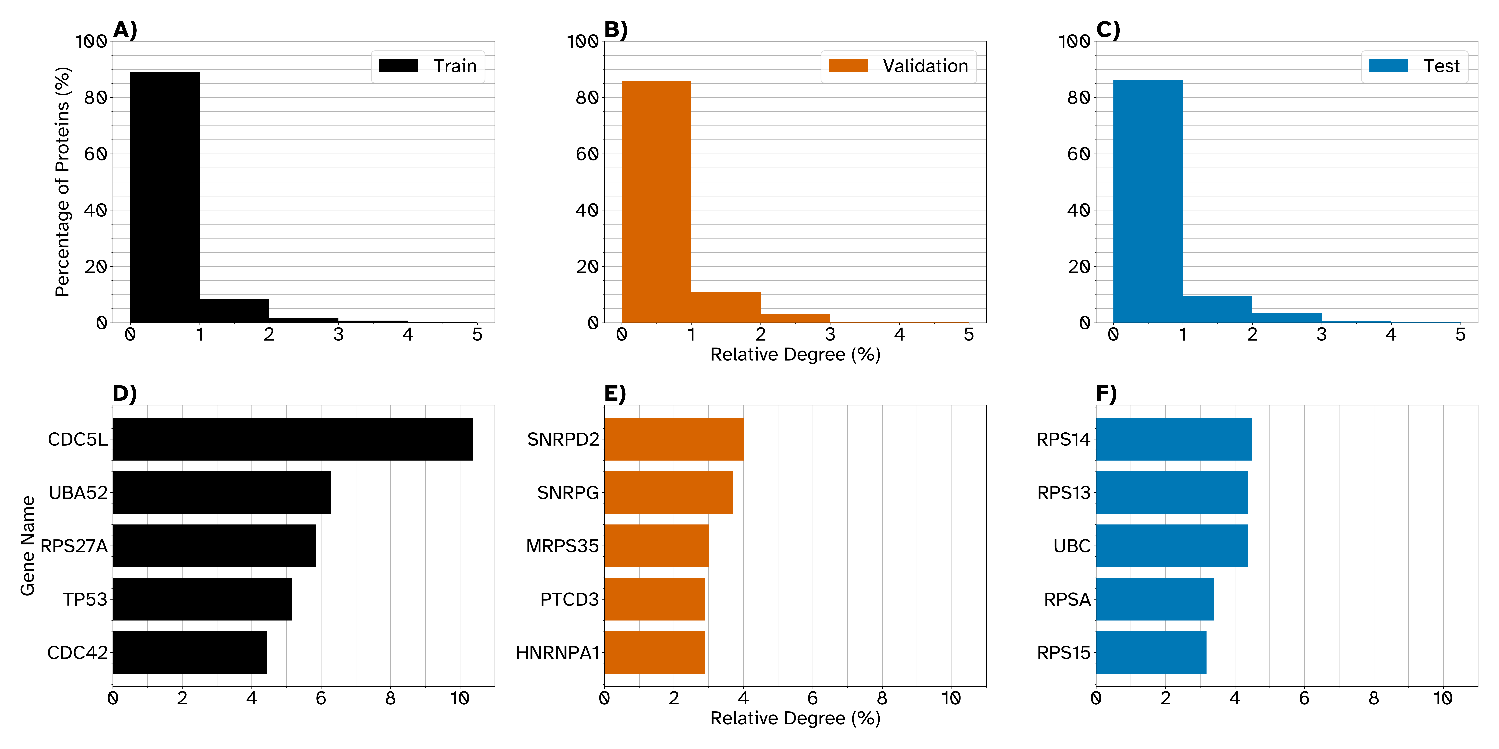
\includegraphics[scale=0.30]{figures/rapppid/rapppid_supp1.png}}
	\caption[Relative Degree of Proteins in the \textit{H. sapiens} \textsc{string} \textsc{c3} dataset.]{\textsf{\textbf{Relative Degree of Proteins in the \textit{H. sapiens} STRING C3 dataset.}} The
distribution of the relative degree of proteins between the three splits of the \textit{H. sapiens} \textsc{string} \textsc{c3} datasets reveal that the vast majority of proteins have a relative degree of less than 1\% \textbf{(A-C)}. The top five proteins with the highest relative degrees are plotted in bar graphs D through F. \textit{CDC5L} has a relative degree of 10.37\%, the highest of the entire dataset. Many of the proteins of high relative degree belong to the families of ribosomal or ribonucleoproteins.}\label{fig:rapppid:degree}
\end{figure}

\begin{figure}[h]
	\centerline{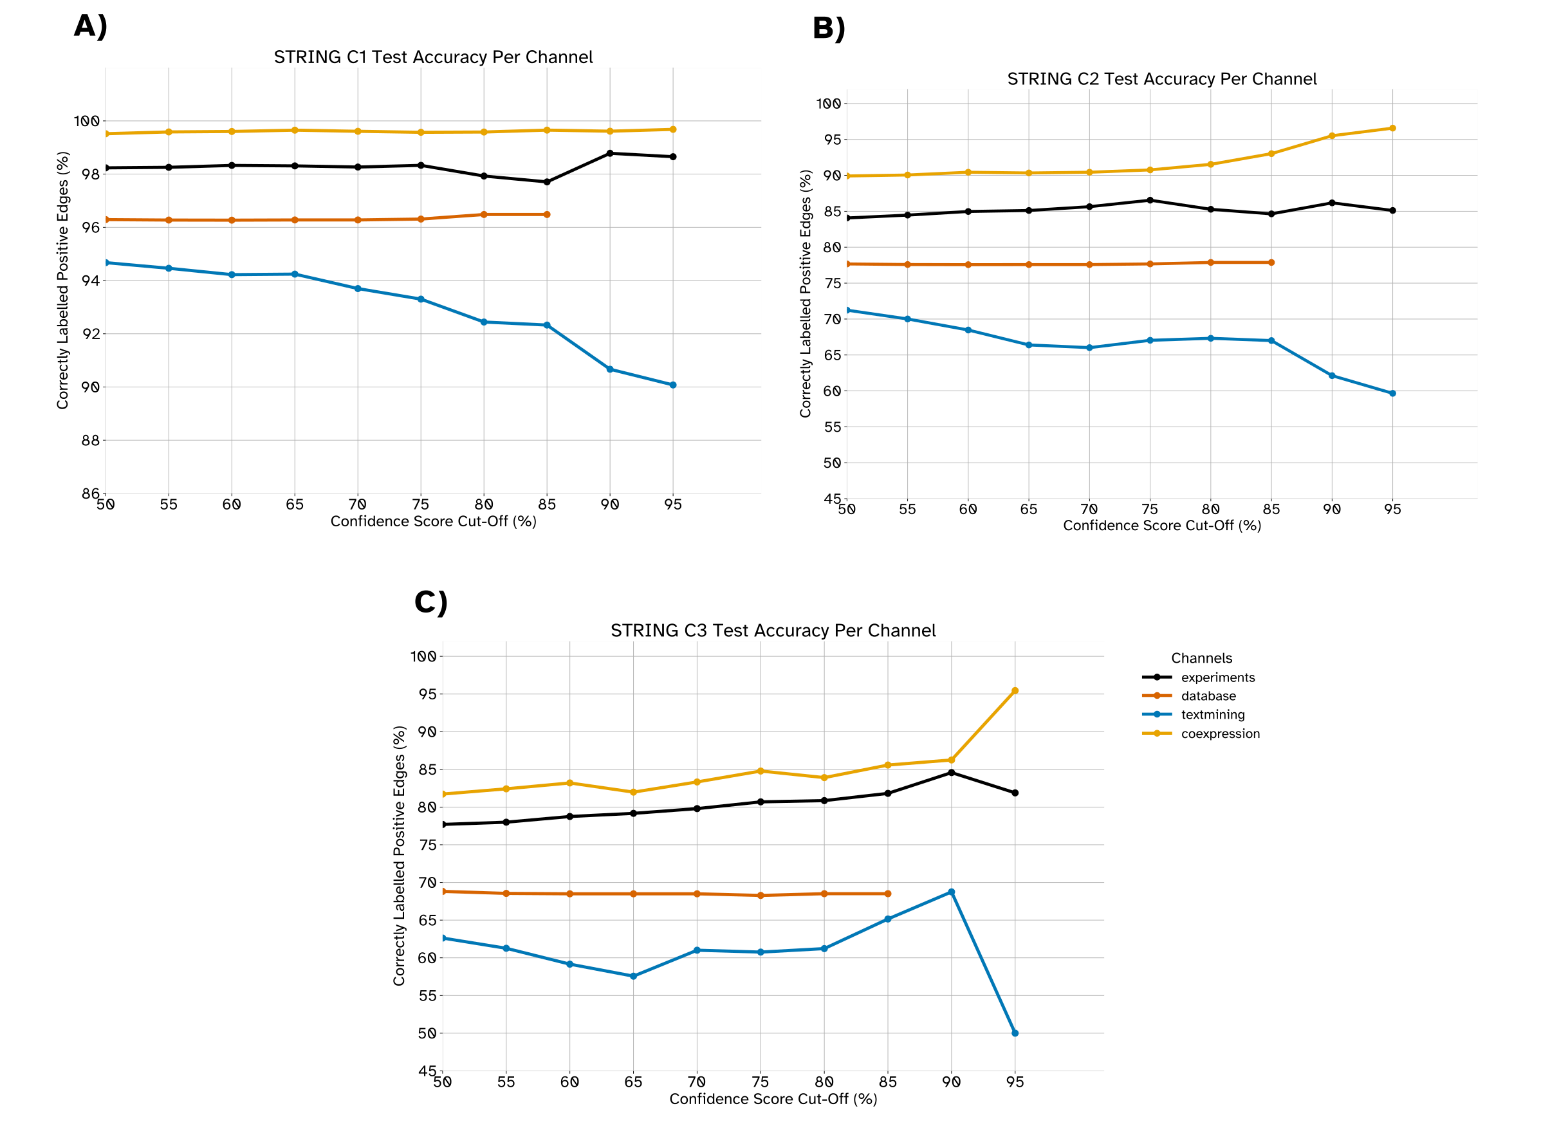
\includegraphics[scale=0.30]{figures/rapppid/rapppid_supp2.png}}
	\caption[Accuracy of positive edges across edge confidence stratified by \textsc{string} channels.]{\textsf{\textbf{Accuracy of positive edges across edge confidence stratified by STRING channels.}} The percentage of correctly labelled positive edges are plotted for each major \textsc{string} channel in the \textsc{c1} \textbf{(A)}, \textsc{c2} \textbf{(B)}, and \textsc{c3} \textbf{(C)} datasets. The x-axis denotes the channel edge confidence cut-off score for each curve’s respective channel.}\label{fig:rapppid:channels_supp}
\end{figure}

\begin{figure}[h]
	\centerline{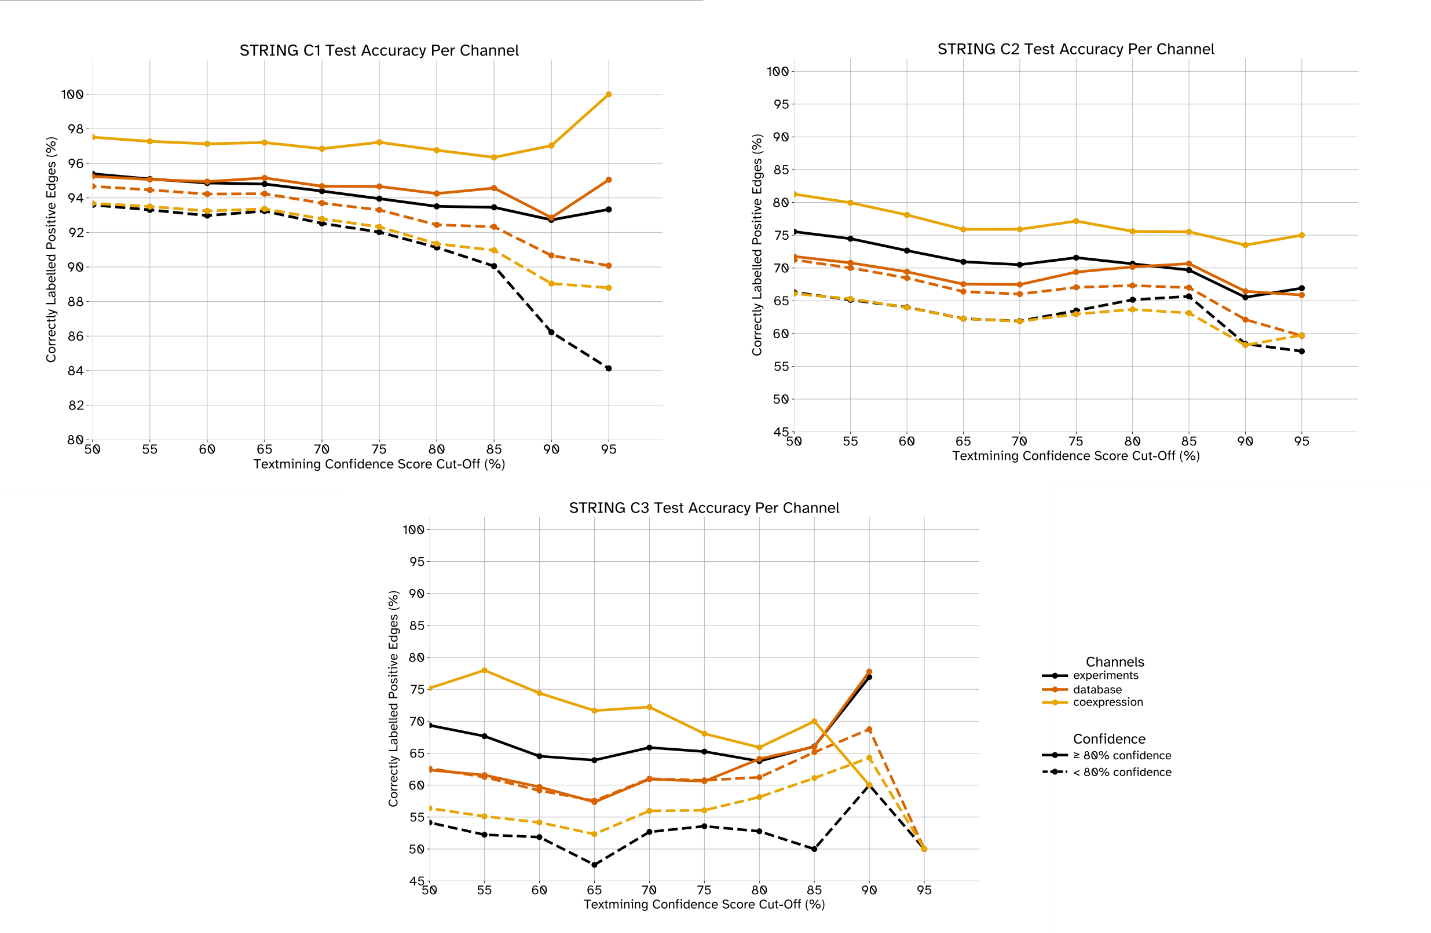
\includegraphics[scale=0.30]{figures/rapppid/rapppid_supp3.png}}
	\caption[Accuracy of positive edges across edge confidence stratified by \textsc{string}
channels.]{\textsf{\textbf{Accuracy of positive edges across edge confidence stratified by STRING channels.}} The percentage of correctly labelled positive edges are plotted for each major \textsc{string} channel, excluding text-mining. Edges are excluded according to the text-mining confidence threshold (x-axis). The solid curves include edges which have a channel confidence $\leq 80\%$ for the channel indicated by the curve’s colour. Dashed curves conversely include edges whose channel confidence is 80\% for the channel indicated by the curve’s colour. Data shown reflects the \textsc{c1} model/dataset in panel \textbf{(A)}, the \textsc{c2} model/dataset in panel \textbf{(B)}, and the \textsc{c3} model/dataset in panel \textbf{(C)}.}\label{fig:rapppid:channels_supp2}
\end{figure}

\begin{figure}[h]
	\centerline{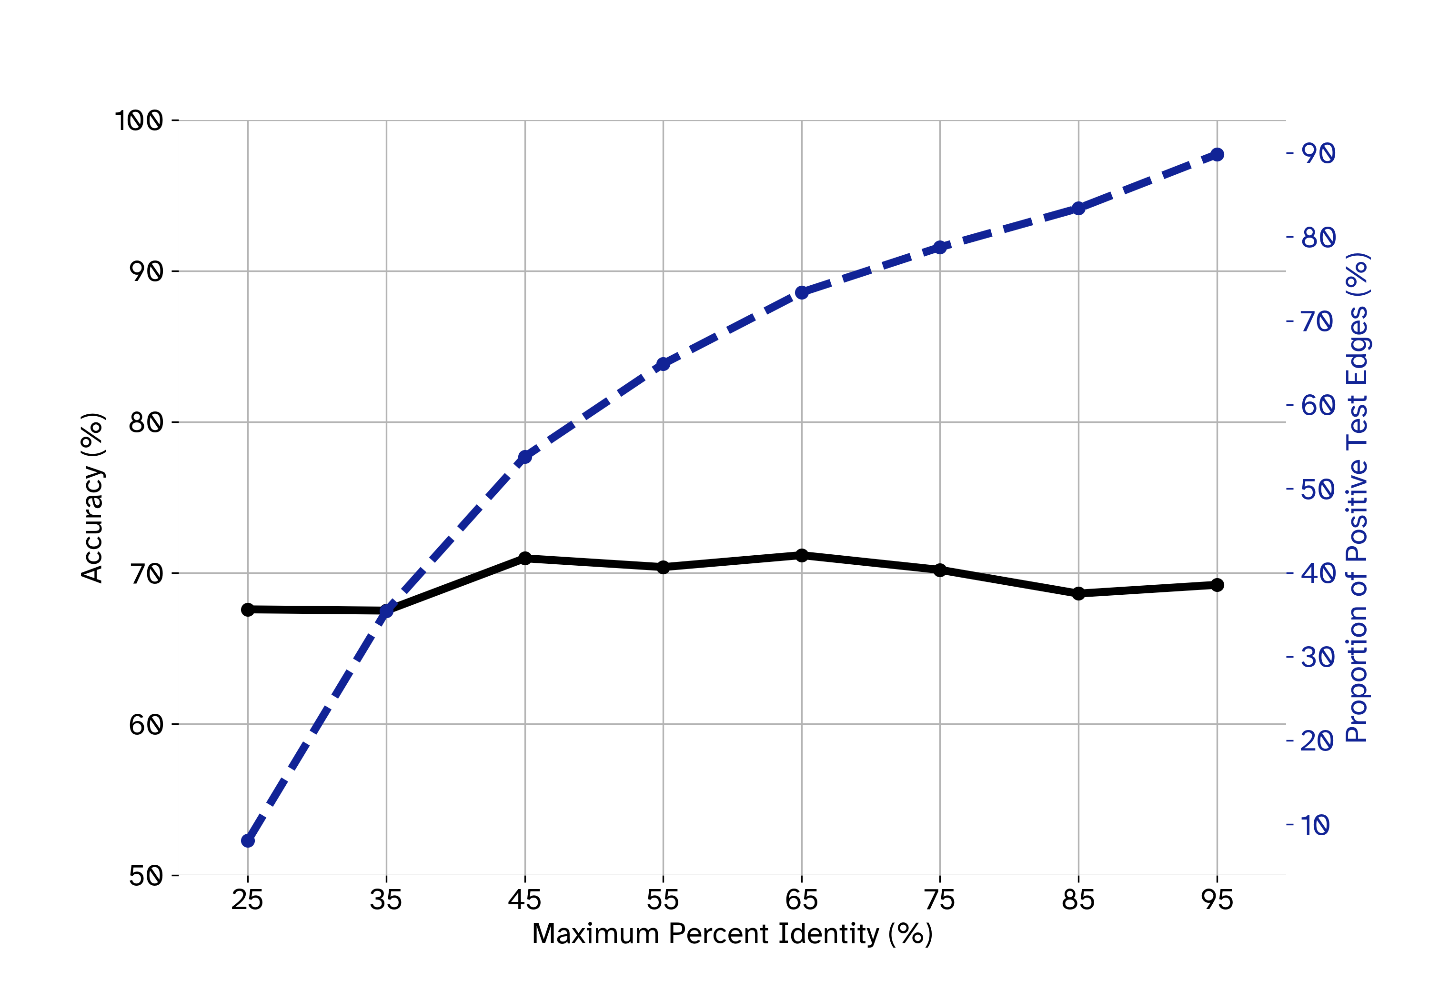
\includegraphics[scale=0.30]{figures/rapppid/rapppid_supp4.png}}
	\caption[Accuracy of positive edges as a function of similarity between testing and
training proteins in \textsc{c3}.]{\textsf{\textbf{Accuracy of positive edges as a function of similarity between testing and training proteins in C3.}} The similarity between testing and training proteins was measured using their percent identity as computed by \textsc{ncbi}'s \textsc{psi-blast} software. The highest percent identity between any training protein and a testing protein in a testing edge was considered to be that testing edge's ``maximum percent identity''. The percentage of accurately labelled positive edges (black curve, left y-axis) is reported for edges with maximum percent identities lower than the threshold reported on the x-axis. The proportion of testing edges for each threshold values is reported by the dashed blue curve and the right y-axis.}\label{fig:rapppid:similarity_supp}
\end{figure}

\begin{figure}[h]
	\centerline{\includegraphics[scale=0.05]{figures/rapppid/rapppid_supp5.png}}
	\caption[Distribution of Interaction Probabilities of Trastuzumab and Pertuzumab with
all Proteins of the Human Proteome as Predicted by \textsc{rapppid}.]{\textsf{\textbf{Distribution of Interaction Probabilities of Trastuzumab and Pertuzumab with all Proteins of the Human Proteome as Predicted by \textsc{rapppid}.}} The probability of interaction between the antibodies (Trastuzumab and Pertuzumab) and each protein in the human proteome (according to \textsc{string}) were individually predicted using \textsc{rapppid}. The distribution of these probabilities is here shown for interactions between Trastuzumab (top) and Pertuzumab (bottom). The quartiles are marked by blue dashed lines, and illustrate that the majority of proteins have a probability of interacting less than 35.9\% and 28.8\% for Trastuzumab and Pertuzumab, respectively. The dotted orange line demarks where \textsc{her2} is positioned in the distribution, holding a probability of interaction of 98.8\% and 95.1\% with Trastuzumab and Pertuzumab, respectively.}\label{fig:rapppid:trastuzumab}
\end{figure}
